\documentclass[border=5mm,
               tikz,
               preview]{standalone}
\usetikzlibrary{arrows.meta, bending, calc, fit, positioning, shapes}

    \begin{document}
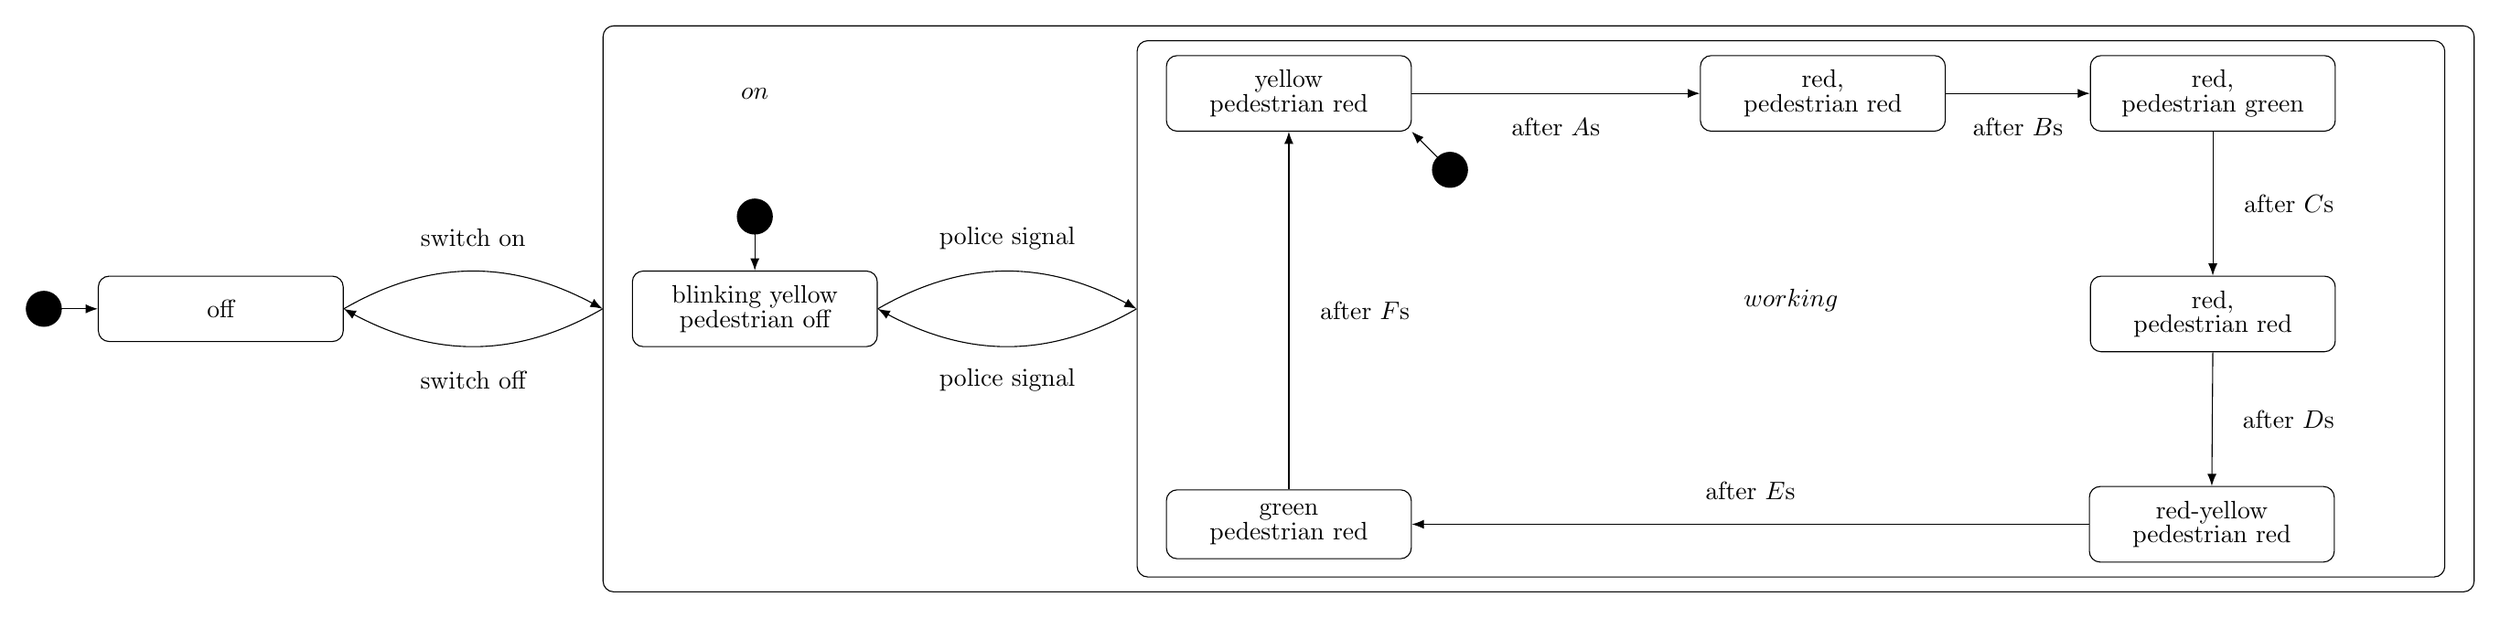
\begin{tikzpicture}[auto,
node distance = 22mm and 17mm,
every node/.style = {draw, rounded corners=1.5mm,
                     inner ysep=2mm, inner xsep=4mm,
                     minimum height=6ex,
%                     font=\bfseries,
                     text width=26mm, align=center},
                    ]
%---
\linespread{0.8}


\node (off) {off};
\node (by) [right=40mm of off] {blinking yellow \\ pedestrian off};
\node (by_a) [draw=none,above=20mm of by] {$on$};
\node (by_d) [draw=none,below=20mm of by] {};
\node (y) [right=40mm of by_a] {yellow \\ pedestrian red};
\node (r_pr) [right=40mm of y] {red, \\ pedestrian red};
\node (r_pg) [right=20mm of r_pr] {red, \\ pedestrian green};
\node (r_pr_2) [below=20mm of r_pg] {red, \\ pedestrian red};
\node (g) [right=40mm of by_d] {green \\ pedestrian red};
\node (ry) [right=94mm of g] {red-yellow \\ pedestrian red};
\node (empty) [draw=none,right=0mm of r_pg,text width=3mm] {};
\node (working) [fit=(y)(r_pr)(r_pg)(r_pr_2)(ry)(g)(empty)] {$working$};
\node (on) [fit=(by)(working)] {};

\coordinate[above=10mm of by]   (temp1);
\coordinate[below right=10mm of y.south east]     (temp2);
\coordinate[left=10mm of off.west]   (temp3);
\path[{Circle[length=5mm,flex]}-{Latex[flex]}]
        (temp1) edge (by)
        (temp2) edge (y.south east)
        (temp3) edge (off.west);
\path[-{Latex[]},bend left]
        (off.east) edge node[draw=none,above] {switch on}  (on.west)
        (on.west) edge node[draw=none,below] {switch off} (off.east)

        (by.east) edge node[draw=none,above] {police signal} (working.west)
        (working.west) edge node[draw=none,below] {police signal} (by.east);
        
\path[-{Latex[]},]
        (y.east) edge node[draw=none,below,text width=13mm] {after $A$s} (r_pr.west)
        (r_pr.east) edge node[draw=none,below,text width=13mm] {after $B$s} (r_pg.west)
        (r_pg.south) edge node[draw=none,text width=13mm] {after $C$s} (r_pr_2.north)
        (r_pr_2.south) edge node[draw=none,text width=13mm] {after $D$s} (ry.north)
        (ry.west) edge node[draw=none,above,text width=13mm] {after $E$s} (g.east)
        (g.north) edge node[draw=none,right,text width=13mm] {after $F$s} (y.south);

%-------
%\node (rotLeft)                             {rotation left};
%\node (rotRight)    [above=of rotLeft]      {rotation right};
%\node (ident)   [fit=(rotLeft)(rotRight)]   {identify};
%
%\node (pause)   [right=of rotRight]          {pause};
%\node (observe) [right= of $(rotLeft.east)!0.5!(rotRight.east)$]
                                            {observe};
%\node (origin)  [right=of rotLeft]          {to origin};
%
%\node (left)    [right=of pause]            {left};
%\node (right)   [right=of origin]           {right};
%\node (neutral) [right=of $(left)!0.5!(right)$] {neutral};
%\node (running) [fit=(left)(right)(neutral)]    {};
%    \node[draw=none,above=7mm of neutral]   {running};
%
%\coordinate[above left=5mm and 2mm of rotLeft.north east]   (temp1);
%\coordinate[above left=5mm and 2mm of pause.north east]     (temp2);
%\coordinate[above left=5mm and 2mm of neutral.north east]   (temp3);
%\path[{Circle[length=2mm,flex]}-{Latex[flex]}, bend left]
%        (temp1) edge (rotLeft.north east)
%        (temp2) edge (pause.north east)
%        (temp3) edge (neutral.north east);
%
%\draw[-{Latex[length=3mm]}]   ([yshift=-1mm] origin.east) -- + (0,3mm);
% edges
%\path[draw, -{Latex[]}, bend left, looseness=1.3]
%        (rotLeft)   edge (rotRight)
%        (rotRight)  edge (rotLeft)
%---
%        (pause.north)   edge[bend right] (ident.north) 
%        (ident.south)   edge[bend right] (origin.south)
%%---
%        (origin.north west)     edge (pause.south west)
%        (pause.south east)      edge (observe.north east)
%%%---
  %      (left)      edge (right)
%        (right)     edge (left)
%
%        (left)      edge (neutral)
%([yshift=1mm] neutral.west) edge ([xshift= 7mm] left.south)
%([xshift=7mm] right.north)   to  ([yshift=-1mm] neutral.west)% exception!?
%        (neutral)   edge (right)
%---
%        (pause)     edge (running)
%        (running)   edge (origin);
\end{tikzpicture}
    \end{document}
